% =====================================================================
% SOEN 6011 -- Deliverable 3 -- Poster
% F2: tan(x) -- Konan Brandon -- 40373534
%
% Compile:  pdflatex poster.tex   (twice)
%
% Digital poster, A0 portrait. Expects ../screenshots/ alongside.
% =====================================================================

\documentclass[final]{beamer}
\usepackage[size=a0,orientation=portrait,scale=1.30]{beamerposter}
\usetheme{Madrid}

\usepackage[utf8]{inputenc}
\usepackage[T1]{fontenc}
\usepackage{graphicx}
\usepackage{amsmath}
\usepackage{booktabs}
\usepackage{tikz}
\usetikzlibrary{mindmap,trees}

\graphicspath{{../screenshots/}{screenshots/}{./}}

\setbeamertemplate{navigation symbols}{}
\setbeamertemplate{headline}{}
\setbeamertemplate{footline}{}
\setbeamercolor{block title}{fg=white,bg=structure}
\setbeamercolor{block body}{bg=black!3}

\title{\huge F2: tan(x) --- Implemented from First Principles}
\author{Konan Brandon \quad ---\quad Student ID 40373534}
\institute{SOEN 6011: Software Engineering Processes ---
           Deliverable 3 --- Summer 2026}
\date{}

\begin{document}

\begin{frame}[t]

% --- Title banner -------------------------------------------------
\begin{beamercolorbox}[wd=\paperwidth,sep=0.6cm,center]{block title}
  \vskip0.3cm
  {\veryHuge\bfseries F2: tan(x)}\\[0.5cm]
  {\Huge Implemented from First Principles}\\[0.6cm]
  {\Large Konan Brandon \quad---\quad Student ID 40373534}\\[0.25cm]
  {\large SOEN 6011: Software Engineering Processes
   \quad$\bullet$\quad Deliverable 3 \quad$\bullet$\quad Summer 2026}
  \vskip0.3cm
\end{beamercolorbox}

\vskip1.5cm

\begin{columns}[t]

% =====================================================================
% LEFT COLUMN
% =====================================================================
\begin{column}{0.315\textwidth}

\begin{block}{The Problem}
  Compute $\tan(x)$ without any library performing the mathematics.
  No \texttt{math} module, no built-in factorial, no built-in
  trigonometry.
  \vspace{0.4cm}

  The constraint is what makes the work interesting: every decision a
  library would have made silently must now be made explicitly, and
  each becomes a requirement that can be verified.
\end{block}

\begin{block}{The Algorithm}
  Maclaurin series for both components of the quotient identity:
  \[ \tan(x) = \frac{\sin(x)}{\cos(x)} \]
  \[ \sin(x) = x - \frac{x^{3}}{3!} + \frac{x^{5}}{5!} - \cdots \]
  \vspace{0.2cm}

  \textbf{No factorial is ever computed.} Dividing one term by its
  predecessor gives the recurrence
  \[ t_{k+1} = t_{k}\cdot\frac{-x^{2}}{(2k)(2k+1)} \]
  which costs one multiplication and one division per term and cannot
  overflow.
  \vspace{0.4cm}

  \textbf{Range reduction.} The tangent has period $\pi$, not $2\pi$,
  because $\sin$ and $\cos$ both change sign and the signs cancel in
  the ratio. Subtracting the nearest whole multiple of $\pi$ confines
  the argument to $[-\pi/2,\ \pi/2]$, where the series converges
  quickly and every asymptote collapses onto a single check.
  \vspace{0.4cm}

  \textbf{Termination by accuracy, not by count.} Summation stops when
  a term falls below $10^{-15}$ --- the point at which it no longer
  changes the result at double precision.
\end{block}




\end{column}

% =====================================================================
% MIDDLE COLUMN
% =====================================================================
\begin{column}{0.315\textwidth}

\begin{block}{A Defect Found by Measurement}
  Testing against a reference at $x = 10^{15}$ returned $-1.557$ where
  the true value is $-1.672$ --- wrong in the first decimal, with no
  error raised.
  \vspace{0.3cm}

  Sampling four thousand angles at each order of magnitude showed
  roughly one significant digit lost per factor of ten:
  \vspace{0.2cm}

  \centering
  \begin{tabular}{lrr}
    \toprule
    \textbf{Magnitude} & \textbf{Typical} & \textbf{Worst} \\
    \midrule
    $10^{2}$ & 13.6 & 10.8 \\
    $10^{4}$ & 11.7 & 8.8 \\
    $10^{6}$ & 9.7 & 6.8 \\
    $10^{8}$ & 7.7 & 5.1 \\
    \bottomrule
  \end{tabular}
  \vspace{0.3cm}

  \raggedright
  Results display ten decimal places. Past $10^{6}$ the worst case
  falls below six correct digits, so the display would present noise as
  precision. \textbf{The validated range is $\pm 10^{6}$}; larger
  angles are refused with an explanation rather than answered.
  \vspace{0.2cm}

  All 636{,}620 exact asymptotes within that range were tested. None
  was missed.
\end{block}

\begin{block}{Unit Testing (PyUnit) --- Problem 8}
  \textbf{58 tests} across eleven classes, each traced to a
  requirement from Deliverable~2. Six of the eleven:
  \vspace{0.3cm}

  \centering
  \begin{tabular}{lr}
    \toprule
    \textbf{Class} & \textbf{Requirement} \\
    \midrule
    Reference angles & TAN-FR-01, 03 \\
    Range reduction & TAN-FR-04 \\
    Undefined points & TAN-FR-07 \\
    Validated range & TAN-FR-11 \\
    Termination & TAN-FR-06 \\
    From-scratch constraint & TAN-FR-02 \\
    \bottomrule
  \end{tabular}
  \vspace{0.4cm}

  \raggedright
  \textbf{Validated by mutation.} Sixteen defects were injected. The
  first version of the suite detected \textbf{seven}; the revised
  version detects \textbf{fourteen}. Both survivors are
  behaviour-preserving.
  \vspace{0.2cm}

  The nine original survivors shared one cause: every tuning constant
  was asserted only relative to itself. Loosening the series tolerance
  degraded accuracy by four orders of magnitude and nothing failed.
  The constants are now pinned to their documented values.
\end{block}

\begin{block}{Quality Tooling --- Problem 7}
  \centering
  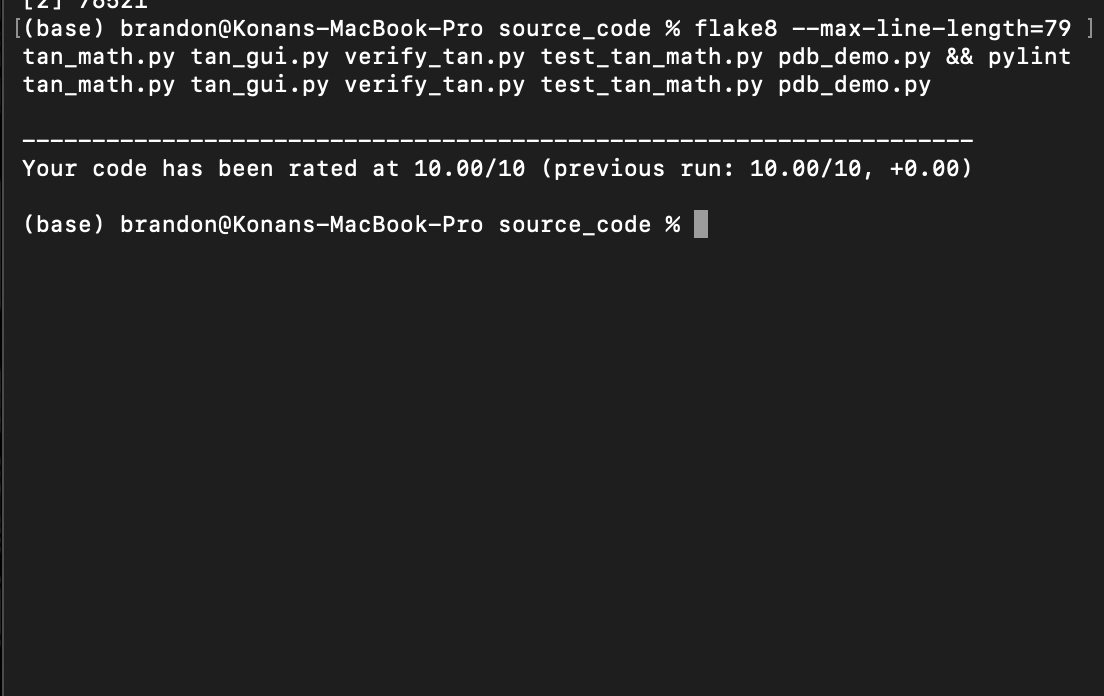
\includegraphics[width=0.97\textwidth]{pylint_score.png}
  \vspace{0.3cm}

  \begin{tabular}{lr}
    \toprule
    Flake8, 79-column limit & no issues \\
    Pylint, all five modules, one combined run & 10.00 / 10 \\
    Unit tests & 58 of 58 \\
    Verification harness & 44 of 44 \\
    \bottomrule
  \end{tabular}
\end{block}

\begin{block}{Debugger: Terms Shrinking to Tolerance --- Problem 7}
  \centering
  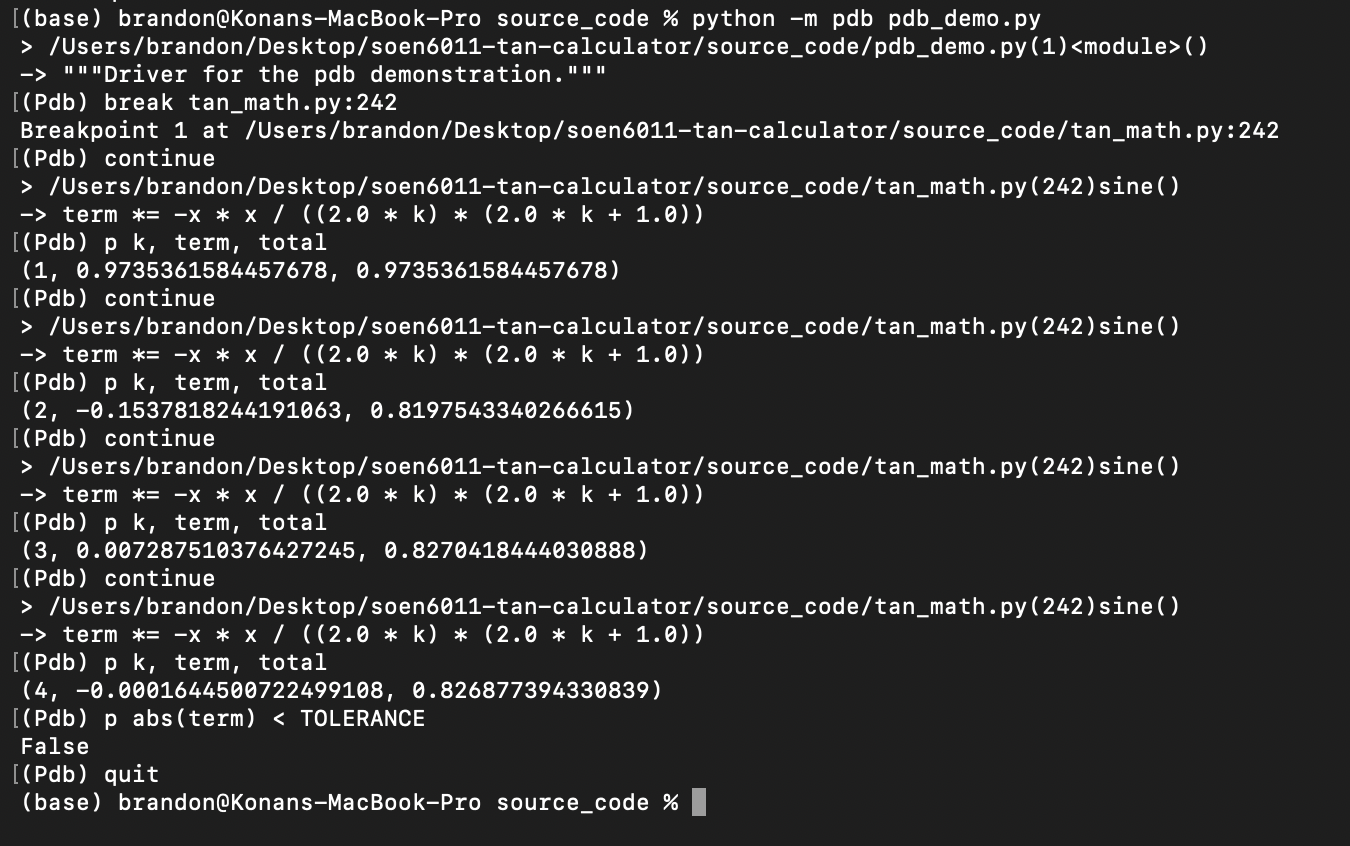
\includegraphics[width=0.97\textwidth]{pdb_02_series_terms.png}
  \vspace{0.2cm}

  \raggedright\small
  Successive terms fall $0.97 \rightarrow 0.15 \rightarrow 0.007
  \rightarrow 0.0001$. The stopping rule is visible rather than
  asserted.
\end{block}

\begin{block}{What the Faults Had in Common}
  Four defects surfaced: silent precision loss at large arguments, a
  signature mismatch between the modules, a documented command that
  failed on a fresh clone, and an unreachable validation branch.
  \vspace{0.2cm}

  \textbf{Every one appeared only when something was run. None was
  visible by reading.}
\end{block}

\end{column}

% =====================================================================
% RIGHT COLUMN
% =====================================================================
\begin{column}{0.315\textwidth}

\begin{block}{Which UI Principles Apply? --- Problem 7}
  \centering
  \resizebox{0.92\textwidth}{!}{%
  \begin{tikzpicture}[mindmap, grow cyclic,
      every node/.style={concept, execute at begin node=\hfil},
      level 1/.append style={level distance=6.5cm, sibling angle=120},
      level 2/.append style={level distance=4.2cm, sibling angle=52}]
  \node [concept, concept color=black!55, text=white]
        {UI\\Principles}
    child [concept color=green!45!black, text=white] {
      node {Applies\\(11)}
      child { node {Error\\diagnosis} }
      child { node {Error\\prevention} }
      child { node {System\\status} } }
    child [concept color=orange!70!black, text=white] {
      node {Reduced\\form (5)}
      child { node {User\\control} }
      child { node {Recognition} } }
    child [concept color=red!60!black, text=white] {
      node {Does not\\apply (2)}
      child { node {Help and\\docs} }
      child { node {Closure} } };
  \end{tikzpicture}}
  \vspace{0.3cm}

  \raggedright\small
  Nielsen's heuristics and Shneiderman's rules were assessed
  individually. Two do not apply: a \textbf{help system} for six
  labelled controls would be evidence the labels failed, and
  \textbf{closure} presupposes a sequence an atomic task lacks.
\end{block}

\begin{block}{Accessibility --- Problem 7}
  The interface aims to be accessible at the level the framework
  permits:
  \vspace{0.2cm}
  \begin{itemize}
    \item Every control carries a visible text label
    \item All functionality reachable from the keyboard; Return
          calculates, Escape clears
    \item Focus begins in the entry field and is visibly indicated
    \item \textbf{Every outcome is stated in words as well as
          colour}, so nothing depends on colour perception
    \item \textbf{Contrast measured on both themes.} No single colour
          can meet 4.5:1 against a light and a dark background --- the
          required luminance ranges do not overlap --- so the palette
          is selected at run time from the theme background. Ratios
          are 6.9--7.1:1 on light and 6.5--7.6:1 on dark, reproducible
          with \texttt{source\_code/check\_contrast.py}
    \item Text wraps rather than clipping; system font settings apply
  \end{itemize}
  \vspace{0.3cm}

  \textbf{Stated limitation.} Screen-reader conformance is not
  claimed: Tkinter exposes no accessibility tree on any platform, so
  WCAG 4.1.2 and 4.1.3 cannot be met within this framework. That is a
  property of Tkinter, and is recorded rather than worked around.
\end{block}

\begin{block}{The Interface}
  \centering
  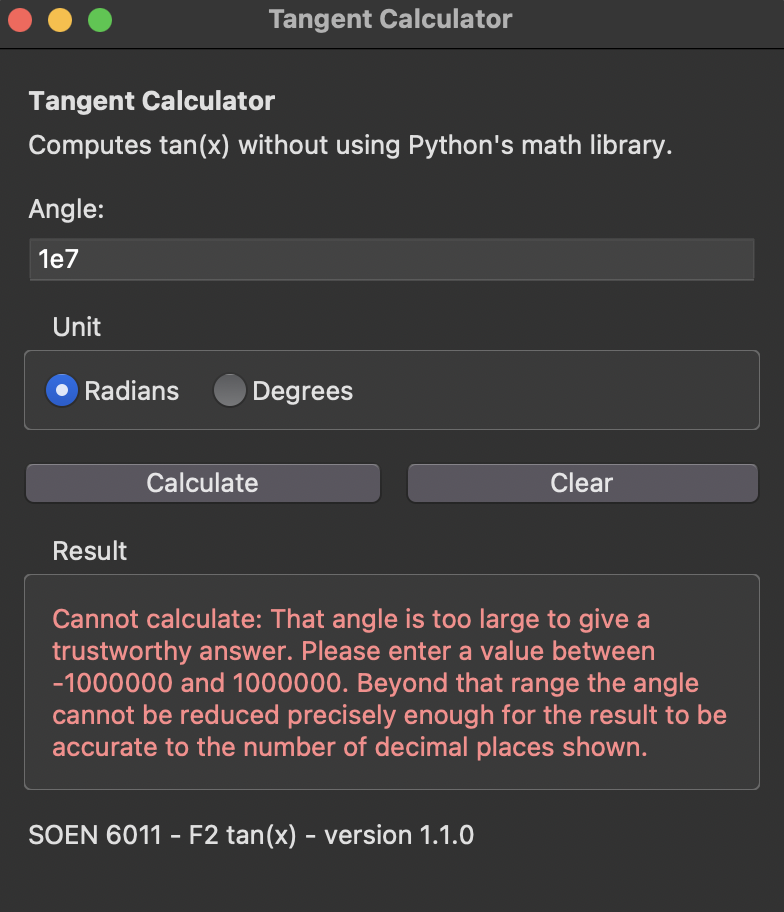
\includegraphics[width=0.72\textwidth]{gui_04_magnitude_guard.png}
  \vspace{0.2cm}

  \raggedright\small
  An angle beyond the validated range, refused with an explanation
  rather than a fault code.
\end{block}



\begin{block}{Generative AI Use}
  Four CASTROFF-structured prompts informed this deliverable: a
  chain-of-thought analysis of which UI principles apply, an
  accessibility audit against WCAG 2.1, a test-suite review, and a
  debugger session design.
  \vspace{0.25cm}

  Two reviews changed the code. The accessibility audit measured the
  colours against a dark theme and found all three below 2:1; the
  palette is now chosen at run time. The test review found nine
  mutations surviving; the suite now catches fourteen of sixteen.
  Prompts and responses are in \texttt{screenshots/}.
\end{block}

\begin{block}{Repository \& Versioning --- Problem 6, 7}
  \centering
  {\small\texttt{github.com/Brand0-code/}}\\
  {\small\texttt{soen6011-tan-calculator}}
  \vspace{0.15cm}

  {\small Version \texttt{v1.1.0} --- Semantic Versioning}
\end{block}

\end{column}

\end{columns}

\end{frame}

\end{document}
